\documentclass{article}
\usepackage[utf8]{inputenc}
\usepackage[danish]{babel}
\usepackage{graphicx}
\font\myfont=cmr12 at 10pt

\title{\huge Software implementation of a personal ECG-scanner \\ \LARGE Assignment 1 \\ \LARGE 02131 Indlejrede Systemer}
\author{Gruppe 1: \\Anna Ølgaard Nielsen, s144437 \\ Van Anh Thi Trinh, s144449 \\ Martin Dariush R. Hansen, s144459}

\usepackage[ddmmyyyy]{datetime}
\newdate{date}{29}{09}{2015}
\date{\myfont \displaydate{date}}

\begin{document}
\maketitle

\newpage

\section*{Abstract}
<<<<<<< HEAD
An ECG shows the electrical activity of the heart. 
=======
An electrocardiography (ECG) shows the electrical activity of the heart and therefore makes it possible to detect QRS complexes, which shows the depolarization of the ventricles in the heart\cite{3}. This paper examines the QRS complexes from an ECG device. This is done by creating a virtual personal ECG scanner coded in C and based on a real-time QRS algorithm, which will filter raw data fetched from a patient, detect the heartbeat from the QRS complexes\cite{1}, and warn the patient if the heartbeat is unstable. Since this is not a real scanner, the raw data is read from a text file, but the processing of it is based on real ECG devices.
>>>>>>> origin/master

\tableofcontents

\newpage
\section{Introduktion}
<<<<<<< HEAD
<<<<<<< HEAD
Vi er tre bachelorstuderende fra softwareteknologi på DTU på tredje semester, der i vores første ud af tre projekter i kurset, 02131 indlejrede systemer, har arbejdet med data fra en ECG Scanner i form af en simuleret hjerterytme. I forbindelse med forløbet, er vi blevet undervist i c, som vi derudfra har anvendt til at skrive et program, der behandler denne data. De overordnede krav til programmets funktionalitet blev givet på forhånd, og der vil i denne rapport fokuseres på tankerne bag programmet og kravene dertil, via en analyse, design og implementering samt slutresultatet med en tilhørende diskussion og konklusion.
=======
Følgende rapport omhandler en ud af tre projekter i kurset, \textit{02131 indlejrede systemer}. Projektet drejer sig om uviklingen af en ECG-scanner, der måler en simuleret hjerterytme. Scanneren filtrerer målingerne, analyserer dem og kan derudfra informere en patient om bl.a. patientens puls. I forbindelse med forløbet, er vi blevet undervist i C, som vi har anvendt til at skrive et program, der kommer til at fungere som en ECG-scanner. De overordnede krav til programmets funktionalitet er givet på forhånd, og der vil i denne rapport fokuseres på tankerne bag programmet og kravene dertil, via en analyse, design og implementering samt slutresultatet med en tilhørende diskussion og konklusion.
>>>>>>> origin/master
=======
Følgende rapport omhandler et ud af tre projekter i kurset, \textit{02131 indlejrede systemer}. Projektet drejer sig om uviklingen af en ECG-scanner, der måler en simuleret hjerterytme. Scanneren filtrerer målingerne, analyserer dem og kan derudfra informere en patient om bl.a. patientens puls. I forbindelse med forløbet, er vi blevet undervist i C, som vi har anvendt til at skrive et program, der kommer til at fungere som en ECG-scanner. De overordnede krav til programmets funktionalitet er givet på forhånd, og der vil i denne rapport fokuseres på tankerne bag programmet og kravene dertil, via en analyse, design og implementering samt slutresultatet med en tilhørende diskussion og konklusion.
>>>>>>> origin/master


\newpage
\section{Arbejdsmetode og samarbejde}
Der er ofte mange måder at løse forskellige problemer på. Vi har i samarbejde taklet disse problemer ved først at lave en brainstorm over mulige løsninger samt deres fordele og ulemper. Derudfra har vi valgt de løsninger, som vi vurderede løste problemet bedst.

Først udviklede vi en samarbejdskontrakt, hvor bl.a. vores ambitioner og samarbejdspolitikker blev formuleret. Vi har arbejdet sammen i de lektioner, som vi har fået til rådighed på DTU, og har flere gange mødtes på andre tidspunkter og arbejdet sammen. En del af arbejdet er blevet delt op imellem os, hvorefter vi hver især har arbejdet med det derhjemme. For at udnytte gruppens ressourcer så godt som muligt, har vi alle lavet noget samtidigt i form af individuel kodeskrivning, pair-programming, individuel rapportskrivning eller gruppediskussioner.

Vi har været gode til at overholde vores aftaler, og der har ikke været problemer med gruppesamarbejdet. Selve koden er skrevet i \textit{Eclipse} og delt gennem \textit{GitHub}, mens rapporten er skrevet og delt gennem \textit{Google Docs} og kompileret med \textit{Latex}.

\section{Analyse}
\subsection{Problemstilling}
For mennesker med hjerteproblemer er det vigtigt at få den rette hjælp, da sådanne problemer i nogle tilfælde kan medføre hjertestop, hvoraf personen kan miste livet. Disse hjerteproblemer opstår ofte uventet, og kan derfor være svære at detektere hos en læge eller på et sygehus, hvor man opholder sig i begrænset tid.

En ECG-scanner måler elektrisk aktivitet og bruges til at måle en persons hjerterytme. Scanneren kan anvendes over længere tidsforløb og er mobil, hvilket gør, at man ikke konstant skal være under opsyn for at kunne få en diagnose på hjerteproblemerne eller få hjælp, hvis man skulle få hjertestop.

ECG-scanneren i sig selv kan dog ikke hjælpe meget uden den rette software til at indlæse data, behandle og fortolke det. Softwaren skal derudover også kunne informere patienten om hjertets tilstand. En tilsynsførende skal også kunne blive alarmeret, hvis der er noget galt. Det er vigtigt, at softwaren gør alt dette i realtid og f.eks. ikke alarmerer lægen for sent. Den tilsynsførende skal også kunne se, om der har været uregelmæssigheder fra besøg til besøg.

Da programmet skal kunne køre på en chip med begrænset hardware og batterilevetid, må det hverken bruge for meget plads eller regnekraft og deraf strøm. Der bør heller ikke blive anvendt datatyper som floats, som bruger relativt meget plads, og ikke er direkte understøttet af alt hardware.

Sidst men ikke mindst er det vigtigt at nævne, at softwaren skal være pålidelig og stabil, og altså altid fungere på samme måde og ikke pludseligt fejle.

\subsection{Afgrænsning}
I den virkelige verden, ville programmet skulle indlæse data fra ECG-scanneren i realtid. I vores tilfælde skal programmet dog blot indlæse data fra en tekstfil, som er blevet udleveret på forhånd. For stadig at virke som om der foretages målinger i realtid, skal programmet ikke indlæse hele tekstfilen på én gang, men én måling skal bearbejdes før den næste indlæses.

Det ville normalt også være et krav at den tilsynsførende og ikke kun brugeren alarmeres, hvis der skulle opstå problemer med hjerterytmen, eller at en ambulance evt. automatisk ville blive sendt ud til patienten. I dette projekt er det dog blot et krav, at det vises på et display, hvis der er hjerteproblemer.

\subsection{Datastrukturer}
<<<<<<< HEAD
En ECG Scanner er et indlejret system, der skal være så effektiv som muligt på begrænset plads. Det er derfor essentielt, hvordan vi opbevarer data fra sensoren. Vi kan forvente 250 samples pr sekund, derfor skal datastrukturen være både hurtig og bruge mindst plads muligt.
=======
En ECG-scanner er et indlejret system, der skal være så effektiv som muligt på begrænset plads. Da et program til en ECG-scanner kan udformes på mange forskellige måder, har vi gjort os en del overvejelser om hvilken løsning, der passer bedst i denne situation.
>>>>>>> origin/master


Vi valgte at implementere vores data som et array med en bestemt størrelse, fordi det er hurtigt at tilgå data i et array, og det har en begrænset størrelse modsat lister som dynamisk array og hægtet liste. Problemet med et begrænset array er, at man ikke kan holde så meget historik ad gangen. Da vi fandt ud af, at historikken var irrelevant udover de værdier filterformlerne benytter, forkortede vi arrayet ned til minimal størrelse.
Arrayet er implementeret som en torus, så når arrayet er fyldt, bliver de ældste data overskrevet med de nye data. Til dette bruger vi modulo, så data ikke bliver indsat uden for arrayet. 
Der blev stadig holdt en samplecounter til hver værdi, der ikke blev nulstillet, som kan bruges til senere beregninger.

Ideen til denne datastruktur fik vi fra tidligere overvejelser om at bruge en kø som datastruktur i stedet. Den har samme princip med at fjerne de ældste data og indsætte ny data. Hvis man implementerede køen som et array, der også fungerede som torus, ville det næsten blive samme løsning, som vi har brugt, bortset fra i en kø, har man kun adgang til den seneste og tidligste værdi, ellers skal man oprette pointers til bestemte værdier. Det så vi som unødvendigt, da man ligeså godt kunne bruge et almindeligt array. Man kunne også implementere køen som en hægtet liste, da det tager meget kort tid at indsætte og slette i en hægtet liste, og man behøver ikke holde pointers. Den hægtet liste vil bare fjerne den bagerste værdi og indsætte den nye værdi forrest, så den hægtede liste vil bevæge sig fremad men med konstant plads. Desværre er det meget tidskrævende at hente andre værdier end den forreste og bagerste. Man kunne godt oprette mange pointers til de steder man ville have, men igen vil det være nemmere at bruge et almindeligt array.
Vi var også omkring dynamiske arrays, men da den opretter nye arrays og flytter alle elementer hver gang arrayet er fyldt, er det både en tidskrævende og pladskrævenede måde at implemetere på.

\subsection{Samples og tidsmåling}
Inputtet, som softwaren modtager fra ECG Scanneren, består af individuelle målinger (samples) for den målte elektriske aktivitet (styrke) af hjertet [ECG]. ECG Scanneren giver 250 samples som output per sekund. Altså er frekvensen:

\begin{equation} 
\frac{1s}{250} = 0,004s
\end{equation}

Hver gang en sample indlæses, forøges en optællings-integer med én. På denne måde kan en sample betragtes som et punkt med en bestemt styrke til en given tid. Idet integers ikke kan indeholde uendeligt store tal, vil denne optæller på et tidspunkt gå i overløb. Det antages at den anvendte chip kan anvende 32-bit integers. Heraf vil der gå så meget tid inden variablen vil have overløb, hvis det antages, at det er en unsigned int:

\begin{equation}
\frac{2^{32}}{250} = 17.179.869 sekunder \approx 200 dage
\end{equation}

Det vurderes, at 200 dage er en tilstrækkelig levetid for programmet, idet det antages at programmet enten genstartes, når batteriet skal oplades/udskiftes, eller ved hvert lægecheck. Alternativt kunne man sætte værdien til 0, inden overløbet finder sted.

\subsection{Indlæsning af Data}
Det er et krav, at man kun får en sample at arbejde med ad gangen, da det er sådan det kommer til at foregå på en rigtig patient. Der er givet en tekstfil med alle målingerne, men der skal altså kun indlæses én måling ad gangen. Hver gang en måling indlæses, indlæses værdien på linjen i tekstfilen, som patienten er nået til. For at læse en bestemt linje er scanneren, som indlæser værdier fra filen, nødt til at læse alle linjerne ned til den ønskede linje. Da dette tager længere tid jo flere målinger der har været, indlæses alle værdierne i stedet med det samme og gemmes i censoren. Hver gang funktionen getNextData kaldes fra main-funktionen, returneres dog kun én værdi og det virker derfor stadig som om at censoren kun har indlæst en enkelt ny værdi som returneres til main-funktionen, der derefter kan sende værdien til filtrering.

\subsection{Filtre}
Dataen behandles via filtre. Low og high-pass filtre fjerner støj i områder i dataen som på baggrund af frekvens eller amplitude adskiller sig fra, hvordan hjerteslag normalt ser ud i dataen. Andre filtre gør det nemmere for programmet at identificere hjerteslagene ved at forstærke og udglatte dataen. Filtrenes formler er givet på forhånd i deres rene (ikkeimplementerede) form, og formlerne udledes eller forklares ikke i denne rapport. En gennemgang af alle filtrene med grafiske fremstillinger kan ses i bilaget.

\subsection{Peakdetektion}
Efter filtreringen detekteres højdepunkterne (peaks) i dataen, hvormed programmet vurderer om højdepunkterne kan betragtes som hjerteslag eller ej. Et forslag til en måde at gøre dette på er givet på forhånd i form at et flowchart. Flowchartet giver også et forslag til, hvordan programmet kan afgøre, om der er problemer med hjerterytmen eller om der er hjertestop. Disse forslag anvendes i vores program.

\subsection{Output}
Når en R-Peak er detekteret, skal patienten kunne se det med det samme, med oplysning om intensiteten af den fundne R-Peak og på hvilket tidspunkt den blev detekteret. Derudover skal patienten også kunne se hvor lang tid der er gået fra den sidst-detekterede R-Peak - RR-intervallet. Patienten skal også kunne se sin puls og advares hvis en R-Peak har en intensitet på under 2000 eller hvis der i træk har været fem RR-intervaller, som ikke har ligget inden for et bestemt interval.

\section{Design}
\begin{figure}[h]
	\centering
	\includegraphics[scale=0.7]{diagram.png}
	\caption{Flowchart for QRS-algoritmen}
\end{figure}

Vores program består af en main.c og tre andre c-filer, Peaks.c, Filter.c og Sensor.c, som main.c har adgang til via deres header-filer. 

\subsection{Sensor}
I Sensor.c opretter vi et file-objekt, der læser en sample ad gangen fra den udleverede ECG.txt fil, der indeholder simulerede data fra en sensor. Hvis næste sample ikke er tom, bliver der scannet et nyt sample ind som main.c får adgang til, ved at kalde getNextData() funktionen.

\subsection{Filtre}
Filter.c består af 5 lag filtre, Low-pass, High-pass, Derivative, Squaring og Moving Window Integration. Det fungerer på den måde, at Low-pass henter rådata fra main.c og giver resultaterne videre til High-pass. High-pass læser resultaterne fra Low-pass ind og giver resultaterne videre til Derivative filteret. Dette fortsætter indtil det bestemte sample er kommet igennem alle 5 filtre, hvorefter det bliver sendt tilbage til main.c, der printer det som en del af outputtet.

I hver af formlerne beskriver x inputtet i den aktuelle funktion, og y beskriver den resulterende værdi, efter det bestemte sample er kørt igennem filteret.

Low-pass filteret:
$$y_n=2y_{n-1}-y_{n-2}+\frac{1}{32}\cdot(x_n-2x_{n-6}+x_{n-12})$$
 
Low-pass filteret filtrerer alle frekvenser over 12 Hz fra og lader kun de lave frekvenser komme igennem.

High-pass filteret:
$$y_n=y_{n-1}-\frac{x_n}{32}+x_{n-16}-x_{n-17}+\frac{x_{n-32}}{32}$$

High-pass filteret filtrerer alle frekvenser under 6 Hz fra og lader kun de høje frekvenser passere. På denne måde har vi kun målinger mellem 6 og 12 Hz tilbage, som bliver sendt videre til derivative filteret.

Derivative filteret:
$$y_n=\frac{1}{8}\cdot(2x_n+x_{n-1}-x_{n-3}-2x_{n-4})$$

Derivative filteret forstærker signalerne, så det er nemmere at detektere peaks senere hen. Desuden flytter den hele grafen til at ligge ved y = 0, når der ikke er detekteret nogle udslag.

Squaring filteret:
$$y_n=x_n^2$$

Squaring filteret kvadrerer inputtet, af den grund at små forskelle bliver større og nemmere at se, og alle signaler bliver positive. Det gør det også nemmere at detektere peaks senere, så man ikke skal tage højde for negative peaks.

Moving Window Integration filteret:
$$y_n=\frac{1}{N}\cdot(x_{n-(N-1)}+x_{n-(N-2)}+...+x_n)$$

Moving Window Integration filteret gør signalet mere jævn. Det er en fordel, da man bedre kan se, hvordan hjerterytmen slår og bevæger sig. Det er angivet at N har værdi 30.

\subsection{Peaks}
Den generelle tanke ved at detektere peaks er, at man finder et toppunkt: $x_{n-1} < x_n > x_{n+1}$. Dette gør så at vi ikke detektere “bløde” peaks, hvor følgende ville gælde: $x_{n-1} \leq x_n \leq x_{n-1}$.

For at detektere peaks har vi brugt QRS-algoritmen, som ses som flowchart nedenfor:
\begin{figure}[h]
	\centering
	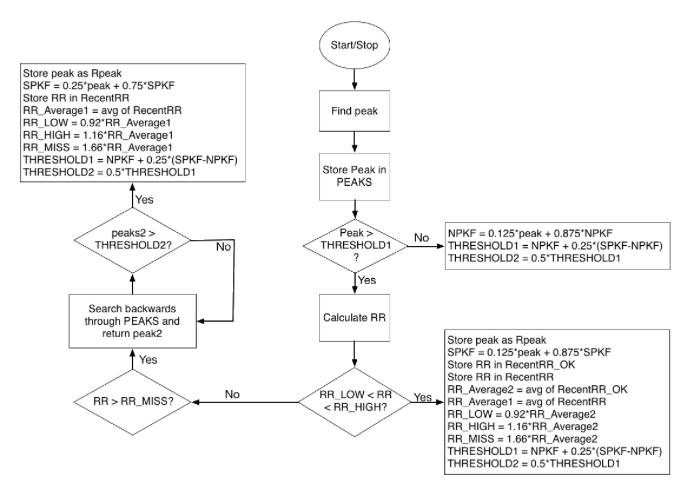
\includegraphics[scale=0.45]{QRS-diagram.png}
	\caption{Flowchart for QRS-algoritmen}
\end{figure}

Man finder først en peak, hvor det gælder at $x_{n-1} < x_n > x_{n+1}$. Derefter tjekker vi om peaket er større end threshold 1, som er en threshold der adskiller noise fra peaks. Hvis peak’en ikke er større end threshold 1, må det ikke være en R-peak med bare noget støj. Derfor bliver NPKF reguleret, da den holder støj-værdien. Efterfølgende bliver både threshold 1 og 2 reguleret ud fra NPKF. Hvis det detekteret peak er større end threshold 1 må det være en R-peak. Vi udregner afstanden fra denne R-peak til den forrige R-peak, og tjekker om den ligger inden for intervallet mellem $RR_{LOW}$ og $RR_{HIGH}$. Hvis dette er tilfældet er det en normal R-peak, og alle variable bliver reguleret efter denne R-peak. Hvis R-peaken ikke ligger inden for intervallet, tjekker vi om dens interval er større end $RR_{MISS}$, der så kan indikere om der måske er hjertestop. Hvis intervallet for R-peaken ikke er større end $RR_{MISS}$ bliver den bare ikke brugt til noget, og algoritmen går i gang med næste detekteret peak. Hvis den interval derimod er større end $RR_{MISS}$, så søger den igennem de seneste peaks, og tjekker om en af dem er større end threshold 2, og hvis den er bliver den peak kategoriseret som en unormal R-peak. På den måde kan vi både detektere hjertestop og uregelmæssigheder i ens hjerterytme. 
Der udstedes en advarsel til brugeren, hvis 5 R-peaks i træk overstiger $RR_{MISS}$, og hvis der detekteres en peak med en værdi mindre end 2000.

\section{Implementering}

\subsection{Indlæsning af data}
Målingerne læses i filen ’sencor’, som indlæser en tekstfil med én måling pr. linje. Da ’sencor’ skal fungere, som en sensor, som måler én måling ad gangen, kan alt data ikke indlæses på samme tid, men skal indlæses løbende. Derfor indlæses hele tekstfilen i stedet for i et array med én værdi pr. indeks, men når funktionen getNextData i ’sencor’  kaldes, må kun én værdi gives videre. En tæller holder derfor styr på nummeret på målingen, som patienten er nået til, så hver gang getNextData kaldes, returneres den værdi i arrayet, som svarer til det, som tælleren angiver. Derefter vokser tælleren med én, så målingen fra næste indeks i arrayet kan returneres næste gang getNextData kaldes. Denne måling gemmes i et array ’data’, som indeholder de nyeste målinger. Målingen filtreres derefter før den næste måling hentes.

\subsection{Filtrering}
Filtreringen af den målte data foregår i en separat fil med en funktion for hver filtrering. Til hver filtrering er også oprettet et array, som skal holde på de nyeste målinger, som er filtreret af det tilhørende filter – f.eks. holder ’lowPass’-arrayet på den nyeste data, der er blevet filtreret gennem Low-pass-filtret. Hvert array har forskellig længde afhængig af hvor mange værdier det næste filter har brug for. For at filtrere en værdi i Derivative -filteret, er der f.eks. kun brug for den nyeste måling og 2., 4., og 5. nyeste måling. Derfor behøver filtreringen før kun at gemme de fem nyeste målinger, og arrayet har derfor længden 5.
Hver filter-funktion bliver kaldt med sit eget tilhørende array som parameter, arrayet tilhørende filteret lige før den, de to arrays længder og nummeret på den nyeste måling – ’lowpass’-funktionen, der tager imod den rå data, får udover ’lowpass’-arrayet, arrayet ’data’ i stedet for et array med filtreret data. I filter-funktionerne bruges data fra arrayet tilhørende den tidligere filtrering til at beregne ny data, som gemmes i dens eget array. Når et array er fyldt ud, overskrives de gamle værdier blot med de nye værdier med start i indeks 0 igen. Arraylængderne bruges her til at sikre at værdierne ligger i den rigtige rækkefølge. F.eks. sikres der, at når værdien før værdien i indeks 0 skal bruges – dvs. uden for arrayet -  hentes den sidste værdi i arrayet i stedet.

\subsection{Peak Detektion}
Peak detection foregår også i en separat fil ’peaks’ med de to funktioner ’findPeaks’ og ’findRPeaks’. Fra main-funktionen kaldes efter filtreringen på ’findPeaks’, der som navnet siger, finder peaks. Funktionen tager som parametre den helt filtrerede data i et array ’mwi’, nummeret på målingen, et array til tiden (nummeret på målingen) og et array til ‘rPeaks’. ’mwi’ indeholder de tre nyeste filtrerede målinger, og med nummeret på målingen kan funktionen beregne om den nyeste måling ligger i indeks 0, 1 eller 2. Når denne er fundet, findes målingen, lige før den, og der tjekkes om denne er større end de to andre værdier. Hvis den er større, er dette et peak og den gemmes i ’peaks’-arrayet, mens målingens nummer gemmes i ’time’-arrayet. Der kaldes derefter på funktionen ’findRPeaks’, der som parametre tager ’time’-arrayet og et array til R-Peaks ’rPeaks’.
I ’findRPeaks’ undersøges først om den nyeste peak i ’peaks’-arrayet er større end grænsen ’threshold1’. Er dette tilfældet undersøges der om RR-intervallet – der er tiden fra sidste fundne R-Peak til nyeste fundne peak - ligger mellem værdierne rrLow og rrHigh. Hvis den gør det, er den nyeste fundne peak en R-Peak, og den gemmes i ’rPeaks’-arrayet. Alle værdierne, der bruges til at finde R-Peaks opdateres derefter som angivet i Design-afsnittet. Hvis RR-intervallet ikke ligger mellem ’rrLow ’ og ’rrHigh ’, undersøges i stedet om den er større end værdien ’rrMiss’. Er den det, søges baglæns i ’peaks’-arrayet fra den nyeste peak for at finde en peak der er større end ’threshold2’, der så er en R-Peak, som skal gemmes i ’rPeaks’-arrayet. Igen opdateres værdierne, som bruges til at finde R-Peaks. Er RR-intervallet ikke større end ’rrMiss’ er en R-Peak ikke fundet, og der sker intet. Hvis RR-intervallet ikke er større end ’threshold1’, opdateres værdierne for ’npkf’, ’threshold1’ og ’threshold2’, og den fundne peak er heller ikke her en R-Peak.  Til sidst returnerer funktionen -1 hvis en R-Peak ikke blev detekteret og nummeret på R-Peak’en, hvis en R-Peak blev detekteret. Denne værdi returneres til ’findPeaks’-funktionen, som sender den videre til ’main’-funktionen, der på denne måde ved om en R-Peak er blevet fundet eller ej, og også hvilken plads i arrayet den ligger på, hvis det er tilfældet at en R-Peak blev fundet.
 
Værdierne til at detektere R-Peaks opdateres løbende, som peaks detekteres, men er i starten defineret ud fra gæt. Estimatet SPKF sættes i starten til 4000 vurderet ud fra de høje peaks værdier på figur x. NPKF vurderes til 1500 ud fra figur y, da der under denne værdi findes peaks, som bør klassificeres som støj. rrAvg1 og rrAvg2 sættes til 151, da dette omtrent er afstanden mellem to R-Peaks. Resten af værdierne: threshold1, threshold2, rrMiss, rrLow og rrHigh kan nu beregnes ud fra estimaterne.

I peaks.c anvendes statiske variabler, da det ikke ønskes, at variablerne skal reinitialiseres, hver gang funktionen kaldes. Da variablerne ikke anvendes uden for funktion, og deraf ikke skal gemmes flere gange, vil de ikke bruge mere hukommelse end nødvendigt hukommelse. Alternativt kan man initialiserer variablerne i main.c, og give variablerne som parametre til funktionen. Dette ville også bruge lidt hukommelse.

\subsection{Output}
Når en R-Peak er fundet meddeles den til patienten, som output sammen med tiden hvor den opstod. Denne beregnes ved at dele nummeret på målingen med 250, idet der måles 250 samples pr. sekund. Pulsen beregnes ved [ASK ANNA].
I ’peaks’-filen holder tælleren ’warningCounter’ ’øje med, om RR-intervallet ligger mellem ’rrLow’ og ’rrHigh’, da den i denne situation altid sættes til 0 uanset hvad den før skulle ligge på. Ligger RR-intervallet ikke mellem ’rrLow’ og ’rrHigh’, vokser den med værdien 1, og kommer den på et tidspunkt op på 5 – altså har den ikke været mellem ’rrLow’ og ’rrHigh’ fem gange i træk, gives en advarsel til patienten.
Hvis en fundet R-Peak har en værdi, der er mindre end 2000 gives også en advarsel.

\section{Resultater}

\subsection{Performance køretider}
Vi har lavet en gprof-profilering af vores færdige system, hvor det store datasæt (ECG10800K.txt) med 10,800,000 samples er blevet brugt, for at få bedst mulig profilering. 
Nedenfor ses en tabel med tidsfordelingen af de fire c-filer, og hver af deres funktioner.
På grund af computerens flere processorer, som alle bruger CPU’en, kører samtidigt, gør dette at resurserne til programmet varierer, og derved varierer profileringen også. Derfor har vi lavet 4 sæt profileringer, og tabellen nedenfor er gennemsnittet af de 4 sæt profileringer.

\begin{table}[h]
	\centering
	\caption{Tidsfordeling for c-filer}
	\begin{tabular}{|c|c|c|c|}
	\hline
	Main.c & Sensor.c & Filter.c & Peaks.c \\ \hline
	0,070 s & 0,095 s & 2,248 s & 0,070 s \\ \hline
	\end{tabular}
\end{table}

\begin{table}[h]
	\centering
	\caption{Tidsfordeling i Filter.c}
	\begin{tabular}{|c|c|c|c|c|}
	\hline
	lowPass & highPass & derivaive & squaring & movingWindow \\ \hline
	0,158 s & 0,253 s & 0,145 s & 0,443 s & 1,588 s \\ \hline
	\end{tabular}
\end{table}
\begin{table}[h]
	\begin{minipage}{.5\linewidth}
		\centering
		\caption{Tidsfordeling i Sensor.c}
		\begin{tabular}{|c|c|}
		\hline
		getNextData & saveData\\ \hline
		0,028 s & 0,068 s \\ \hline
		\end{tabular}
	\end{minipage}%
	\begin{minipage}{.5\linewidth}
		\centering
		\caption{Tidsfordeling i Peaks.c}
		\begin{tabular}{|c|c|}
		\hline
		findPeaks & findRPeaks \\ \hline
		0,068 s & 0,003 s \\ \hline
		\end{tabular}
	\end{minipage}
\end{table}

I \textbf{\textit{Bilag 1}} ses der på diagrammet en tidsfordeling af alle vores c-filer. Det ses, at Filter.c bruger 90\% af CPU-tiden, når programmet bliver kørt. 

Da Filter.c bruger størstedelen af CPU-tiden, er det ret relevant at kigge på dens funktioner. I \textbf{\textit{Bilag 2}} ses det, at Moving Window Integration-funktionen bruger 61 \% af CPU-tiden for Filter.c. Hvis man skulle få programmet til at køre hurtigere, ville det nok være smart at effektivisere Moving Window Integration, da den bruger så stor en procentdel af tiden. Dette bliver diskuteret nærmere under diskussionsafsnittet.

\subsection{Filtrerede R-peaks}

\begin{figure}[h]
	\begin{minipage}{.5\linewidth}
		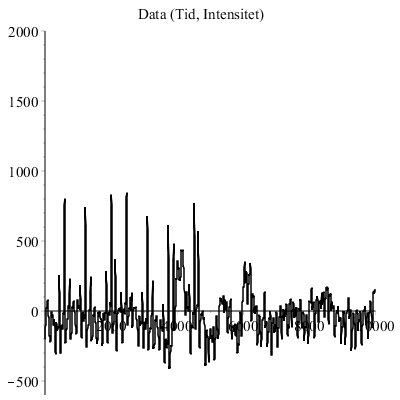
\includegraphics[scale=0.4]{Filter0.png}	
		\caption{Datasæt før filtrering}
	\end{minipage}%
	\begin{minipage}{.5\linewidth}
		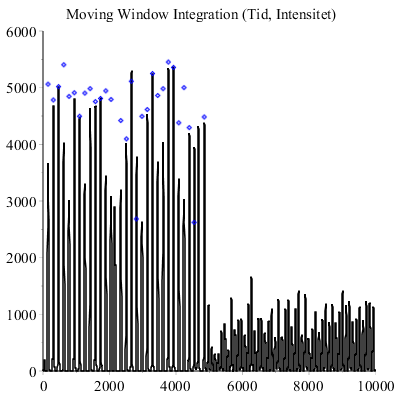
\includegraphics[scale=0.4]{Filter5Peaks.png}	
		\caption{Datasæt efter filtrering}
	\end{minipage}
\end{figure}


\section{Diskussion}

\subsection{Detekterede R-peaks og advarsler}
(Der kommer aldrig advarsler, nogle R-Peaks detekterer vi ikke)

\subsection{Effektivisering af kode}
Under resultatafsnittet sås det, at Moving Window Integration-funktionen brugte størstedelen af CPU-tiden, og det derfor kunne være ret relevant at effektivisere den. 
Det er muligt helt at undgå den for-løkke, der kører 30 gange i movingWindow. Hvis man i stedet for at skulle addere de seneste 30 x-værdier hver gang movingWindow bliver kaldt, kunne man bare gemme summen til næste sample, og bare subtraktere den ældste sample fra summen og addere den nyeste sample til summen. Dette kører i konstant tid frem for lineær tid, og hvis vi havde tid til at gøre dette i vores program, vil vi forvente en markant ændring i CPU-tiden.

\begin{equation}
sum = x_1+x_2+...+x_{30}
\end{equation}

\begin{equation}
sum = sum-x_1+x_{31}
\end{equation}

Det er ret positivt, at det er vores filtre, der bruger al CPU-tiden. Det betyder, at alt andet kodemæssigt kører forholdsvist hurtigt. Filtrene er implementeret næste direkte efter de angivne formler, så udover Moving Window Integration, er det svært at gøre dem bedre. Derved vurderer vi, at vores kode køre hurtigt og effektivt.


\newpage
\section{Konklusion}
Det kan konkluderes, at det er lykkedes at fremstille et program, der indlæser simuleret data fra en tekstfil, filtrerer det og deraf bl.a. fjerner støj fra det og finder toppunkter i dataen, hvorefter det vurderes om der er tale om et hjerteslag. Dertil vurderer programmet, om hjerterytmen er ustabil, og viser relevant data samt alarmbeskeder til brugeren. Udfra profileringen kan det konkluderes, at programmet virker, og at det kører forholdsvis hurtigt.

\newpage
\section{Litteraturliste}
[ECG] http://medical-dictionary.thefreedictionary.com/ECG - 26-09-2015

\newpage
\section{Bilag}
\subsection*{Bilag 1}
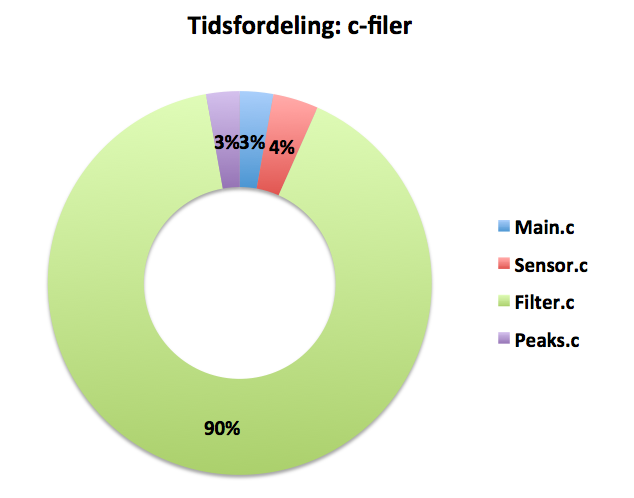
\includegraphics[scale=0.47]{c-filer.png}
\subsection*{Bilag 2}
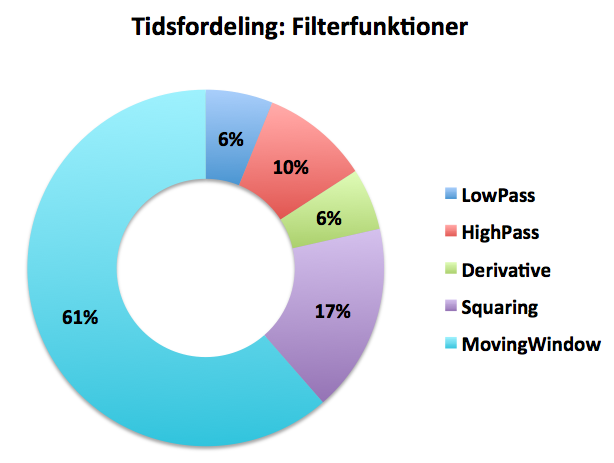
\includegraphics[scale=0.49]{filter-funktioner.png}
\subsection*{Bilag 3}
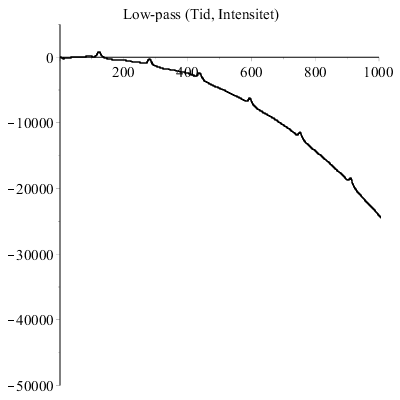
\includegraphics[scale=0.6]{Filter1.png}
\subsection*{Bilag 4}
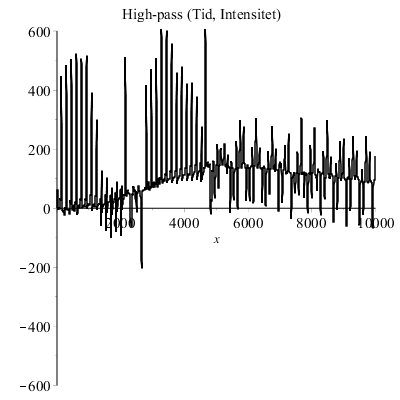
\includegraphics[scale=0.6]{Filter2.png}
\subsection*{Bilag 5}
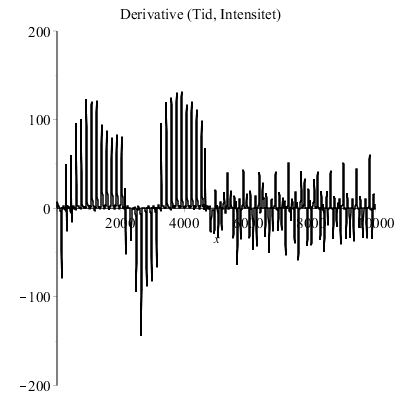
\includegraphics[scale=0.6]{Filter3.png}
\subsection*{Bilag 6}
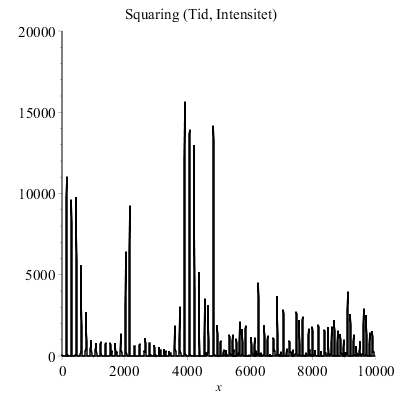
\includegraphics[scale=0.6]{Filter4.png}
\subsection*{Bilag 7}
\includegraphics[scale=0.6]{Filter5close2.png}


\end{document}